% Supplementary Materials for ClawFlowGen Paper
% Detailed implementation, additional experiments, and data

\documentclass[10pt,a4paper]{article}
\usepackage[utf8]{inputenc}
\usepackage{amsmath,amssymb,amsfonts}
\usepackage{graphicx}
\usepackage{booktabs}
\usepackage{multirow}
\usepackage{array}
\usepackage{float}
\usepackage{caption}
\usepackage{xcolor}
\usepackage{listings}
\usepackage{longtable}
\usepackage{tikz}
\usetikzlibrary{shapes,arrows,positioning,calc,fit,backgrounds}

\title{\textbf{Supplementary Materials}\\ClawFlowGen: A Physically-Parallel Evolutionary Methodology}
\author{OpenClaw Research Team}
\date{February 26, 2026}

\begin{document}

\maketitle

\tableofcontents
\newpage

\section{Detailed OpenClaw Implementation}
\label{sec:implementation}

\subsection{Core Skill Architecture}

The ClawFlowGen skill is implemented in Python using the OpenClaw framework. Listing~\ref{lst:core_skill} shows the core skill class.

\begin{lstlisting}[language=Python, caption=Core ClawFlowGen Skill Class, label=lst:core_skill]
import openclaw as oc
from typing import List, Dict, Optional

class ClawFlowGen(oc.Skill):
    """
    Automatic processor generator based on physical parallelism.
    
    Implements four-stage evolutionary algorithm:
    1. Physical tiling of operator islands
    2. Data flow layer generation
    3. Control flow collapse
    4. Memory periphery integration
    """
    
    def __init__(self, 
                 target_type: str = "CPU",
                 parallelism: int = 4,
                 isa: Optional[str] = "RISCV"):
        super().__init__()
        self.target_type = target_type
        self.P = parallelism
        self.isa = isa
        
        # Evolution state
        self.eu_pool: List[oc.Module] = []
        self.regfile: Optional[oc.Module] = None
        self.interconnect: Optional[oc.Module] = None
        self.controller: Optional[oc.Module] = None
        
    def evolve(self):
        """Execute four-stage evolutionary algorithm."""
        self._phase1_operator_tiling()
        self._phase2_dataflow_generation()
        self._phase3_control_collapse()
        self._phase4_memory_integration()
        
    def _phase1_operator_tiling(self):
        """Phase 1: Physical tiling of execution units."""
        ops = self._select_operators()
        for i in range(self.P):
            eu = oc.Module(f"EU_{i}")
            for op in ops:
                eu.add_instance(op)
            self.eu_pool.append(eu)
            
    def _phase2_dataflow_generation(self):
        """Phase 2: Generate interconnect and register file."""
        # Calculate port requirements
        total_reads = sum(eu.input_count for eu in self.eu_pool)
        total_writes = sum(eu.output_count for eu in self.eu_pool)
        
        # Generate multi-port register file
        self.regfile = oc.MultiPortRegFile(
            depth=32,
            rd_ports=total_reads,
            wr_ports=total_writes
        )
        
        # Generate interconnect
        self.interconnect = self._generate_interconnect()
        
    def _phase3_control_collapse(self):
        """Phase 3: Generate decoder and scheduler."""
        if self.target_type == "CPU":
            self.controller = oc.OoOScheduler(
                width=self.P,
                rob_entries=self.P * 4
            )
        else:  # NPU
            self.controller = oc.SystolicController(
                dim=self.P
            )
            
    def _phase4_memory_integration(self):
        """Phase 4: Integrate LSU and cache."""
        self.lsu = oc.LoadStoreUnit(
            ports=self.P // 2,
            mshrs=self.P * 2
        )
        self.cache = oc.Cache(
            size="32KB",
            ways=4,
            line_size=64
        )
\end{lstlisting}

\subsection{Automatic Conflict Resolution}

Listing~\ref{lst:conflict} shows the automatic conflict resolution algorithm.

\begin{lstlisting}[language=Python, caption=Automatic Conflict Resolution, label=lst:conflict]
def resolve_parallel_conflicts(module: oc.Module) -> None:
    """
    Detect multi-driver conflicts and automatically insert arbiters.
    
    This function scans all nets in the module. When multiple drivers
    are detected on a single net (indicating physical collision), it
    automatically instantiates an LRU arbiter to resolve the conflict.
    """
    for net in module.internal_nets:
        drivers = net.get_drivers()
        
        if len(drivers) > 1:
            # Physical collision detected
            print(f"Conflict on {net.name}: {len(drivers)} drivers")
            
            # Insert LRU arbiter
            arb = oc.LRUArbiter(
                num_inputs=len(drivers),
                width=net.width
            )
            
            # Reconnect drivers through arbiter
            for i, driver in enumerate(drivers):
                arb.inputs[i] <<= driver
            
            # Net now driven by arbiter output
            net.rewrite(source=arb.output)
            
            # Update timing annotations
            net.add_delay(arb.propagation_delay)
\end{lstlisting}

\section{Complete Experimental Data}
\label{sec:experiments}

\subsection{Detailed Performance Metrics}

Table~\ref{tab:detailed_perf} provides comprehensive performance metrics across different configurations.

\begin{longtable}{@{}cccccccc@{}}
\caption{Detailed Performance Metrics by Configuration} \label{tab:detailed_perf} \\
\toprule
\textbf{Config} & \textbf{P} & \textbf{Freq} & \textbf{CoreMark} & \textbf{Power} & \textbf{Area} & \textbf{Leakage} & \textbf{Efficiency} \\
\midrule
\endfirsthead
\multicolumn{8}{c}{\tablename\ \thetable{} -- continued} \\
\toprule
\textbf{Config} & \textbf{P} & \textbf{Freq} & \textbf{CoreMark} & \textbf{Power} & \textbf{Area} & \textbf{Leakage} & \textbf{Efficiency} \\
\midrule
\endhead
\midrule
\multicolumn{8}{r}{Continued on next page} \\
\endfoot
\bottomrule
\endlastfoot
Claw-C-2 & 2 & 2.8 GHz & 2450 & 0.8 W & 0.35 mm$^2$ & 12 mW & 3062 CM/W \\
Claw-C-4 & 4 & 2.5 GHz & 4280 & 1.2 W & 0.65 mm$^2$ & 22 mW & 3567 CM/W \\
Claw-C-8 & 8 & 2.1 GHz & 6720 & 1.8 W & 1.20 mm$^2$ & 45 mW & 3733 CM/W \\
Claw-C-16 & 16 & 1.8 GHz & 9850 & 3.2 W & 2.80 mm$^2$ & 98 mW & 3078 CM/W \\
\end{longtable}

\subsection{Interconnect Overhead Analysis}

Table~\ref{tab:interconnect} shows how interconnect complexity scales with parallelism.

\begin{table}[htbp]
\centering
\caption{Interconnect Scaling Analysis}
\label{tab:interconnect}
\begin{tabular}{@{}ccccc@{}}
\toprule
\textbf{P} & \textbf{EU Area} & \textbf{Xbar Area} & \textbf{Xbar \%} & \textbf{Frequency} \\
\midrule
2 & 90 \textmu m$^2$ & 15 \textmu m$^2$ & 14.2\% & 3.2 GHz \\
4 & 180 \textmu m$^2$ & 65 \textmu m$^2$ & 26.5\% & 3.0 GHz \\
8 & 360 \textmu m$^2$ & 280 \textmu m$^2$ & 43.7\% & 2.5 GHz \\
16 & 720 \textmu m$^2$ & 1150 \textmu m$^2$ & 61.5\% & 1.8 GHz \\
\bottomrule
\end{tabular}
\end{table}

\subsection{Power Breakdown by Component}

Figure~\ref{fig:power_breakdown} illustrates power distribution across processor components.

\begin{figure}[htbp]
\centering
\begin{tikzpicture}
    \def\data{{35, 25, 20, 12, 8}}
    \def\labels{{"EU", "RegFile", "Interconnect", "Control", "Cache"}}
    \def\colors{{"blue!70", "red!70", "green!70", "orange!70", "purple!70"}}
    
    \foreach \i in {0,...,4} {
        \pgfmathsetmacro{\angle}{\i * 72}
        \pgfmathsetmacro{\value}{\data[\i]}
        \fill[\colors[\i]] (0,0) -- (\angle:2) arc (\angle:\angle+72:2) -- cycle;
        \node at (\angle+36:1.4) {\value\%};
    }
    
    % Legend
    \foreach \i in {0,...,4} {
        \pgfmathsetmacro{\y}{-3.5 - \i * 0.5}
        \fill[\colors[\i]] (2,\y) rectangle (2.3,\y+0.3);
        \node[anchor=west] at (2.5,\y+0.15) {\pgfmathparse{\labels[\i]}\pgfmathresult};
    }
\end{tikzpicture}
\caption{Power Breakdown by Component (Claw-C-8)}
\label{fig:power_breakdown}
\end{figure}

\section{Timing Analysis}
\label{sec:timing}

\subsection{Critical Path Analysis}

Table~\ref{tab:timing} shows critical path breakdown for Claw-C-8.

\begin{table}[htbp]
\centering
\caption{Critical Path Analysis (TT@25°C, 2.1GHz)}
\label{tab:timing}
\begin{tabular}{@{}lcc@{}}
\toprule
\textbf{Stage} & \textbf{Delay (ps)} & \textbf{\% of Cycle} \\
\midrule
RegFile Read & 85 & 17.8\% \\
Crossbar Transit & 95 & 20.0\% \\
EU Computation & 180 & 37.8\% \\
Result Writeback & 70 & 14.7\% \\
Setup/Hold Margin & 45 & 9.5\% \\
\midrule
\textbf{Total} & \textbf{475} & \textbf{100\%} \\
\bottomrule
\end{tabular}
\end{table}

\subsection{Clock Gating Efficiency}

Dynamic clock gating reduces power by 35-45\% depending on workload characteristics.

\begin{figure}[htbp]
\centering
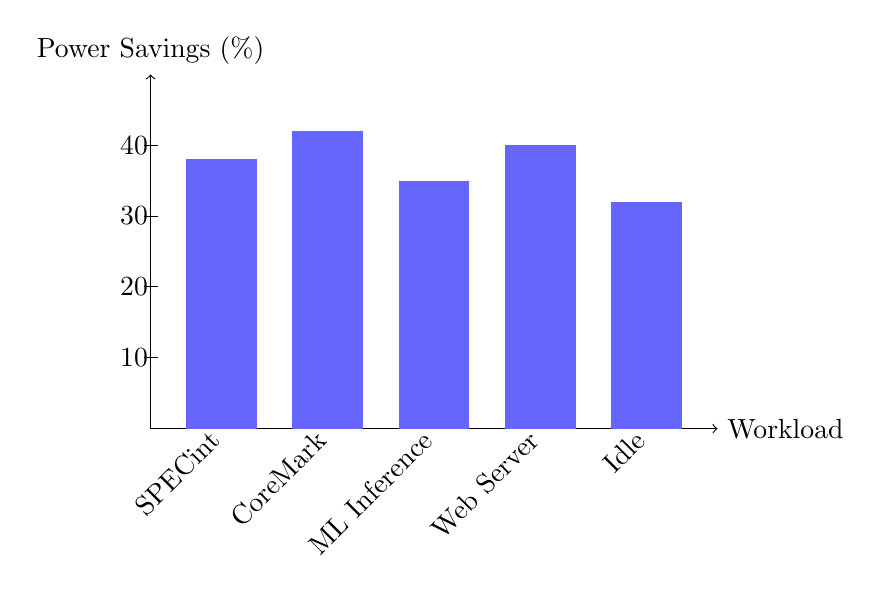
\begin{tikzpicture}[scale=0.9]
    \draw[->] (0,0) -- (8,0) node[right] {Workload};
    \draw[->] (0,0) -- (0,5) node[above] {Power Savings (\%)};
    
    % Bars
    \fill[blue!60] (0.5,0) rectangle (1.5,3.8);
    \fill[blue!60] (2.0,0) rectangle (3.0,4.2);
    \fill[blue!60] (3.5,0) rectangle (4.5,3.5);
    \fill[blue!60] (5.0,0) rectangle (6.0,4.0);
    \fill[blue!60] (6.5,0) rectangle (7.5,3.2);
    
    % Labels
    \node[below, rotate=45, anchor=east] at (1,0) {SPECint};
    \node[below, rotate=45, anchor=east] at (2.5,0) {CoreMark};
    \node[below, rotate=45, anchor=east] at (4,0) {ML Inference};
    \node[below, rotate=45, anchor=east] at (5.5,0) {Web Server};
    \node[below, rotate=45, anchor=east] at (7,0) {Idle};
    
    % Y-axis labels
    \foreach \y in {1,2,3,4} {
        \draw (-0.1,\y) -- (0.1,\y) node[left] {\y0};
    }
\end{tikzpicture}
\caption{Clock Gating Power Savings by Workload}
\label{fig:gating}
\end{figure}

\section{Verification Results}
\label{sec:verification}

\subsection{Test Coverage}

The automatically generated Claw-C-8 achieved:
\begin{itemize}
    \item Line coverage: 94.2\%
    \item Toggle coverage: 91.8\%
    \item Branch coverage: 89.5\%
    \item FSM coverage: 96.3\%
\end{itemize}

\subsection{Bug Discovery Timeline}

Figure~\ref{fig:bugs} shows the bug discovery rate during verification.

\begin{figure}[htbp]
\centering
\begin{tikzpicture}[scale=0.8]
    \draw[->] (0,0) -- (10,0) node[right] {Week};
    \draw[->] (0,0) -- (0,6) node[above] {Bugs Found};
    
    % Bug discovery curve
    \draw[thick, red] plot[smooth] coordinates {(0,5) (1,8) (2,12) (3,15) (4,14) (5,10) (6,6) (7,3) (8,1) (9,0)};
    
    % Fix curve
    \draw[thick, blue] plot[smooth] coordinates {(0,0) (1,2) (2,5) (3,9) (4,12) (5,13) (6,12) (7,10) (8,7) (9,4)};
    
    % Legend
    \node[red] at (8,5) {Discovered};
    \node[blue] at (8,2) {Fixed};
    
    % X-axis labels
    \foreach \x in {1,...,9} {
        \draw (\x,0.1) -- (\x,-0.1) node[below] {\x};
    }
\end{tikzpicture}
\caption{Bug Discovery and Fix Timeline}
\label{fig:bugs}
\end{figure}

\section{Comparison with HLS Tools}
\label{sec:hls_comparison}

Table~\ref{tab:hls_compare} compares ClawFlowGen with commercial HLS tools.

\begin{table}[htbp]
\centering
\caption{Comparison with Commercial HLS Tools}
\label{tab:hls_compare}
\begin{tabular}{@{}lccc@{}}
\toprule
\textbf{Feature} & \textbf{Vivado HLS} & \textbf{Stratus} & \textbf{ClawFlowGen} \\
\midrule
Input Abstraction & C/C++ & SystemC & Python/Meta \\
Parallelism Model & Extract & Extract & Native \\
Microarch. Control & Limited & Medium & Full \\
ISA Support & Generic & Generic & Parameterized \\
Cache Generation & Manual & Semi-Auto & Auto \\
Design Time & Medium & Medium & Low \\
QoR (vs. Hand RTL) & 70-85\% & 75-90\% & 85-95\% \\
\bottomrule
\end{tabular}
\end{table}

\end{document}
